\section{Distributed Shared Memory}

Applications written for \Grappa utilize two forms of memory: local and
global. Local memory is local to a single core within a node in the system.
Accesses occur through conventional pointers. The compiler emits an access and
the memory is manipulated directly. Applications use local accesses for a
number of things in \Grappa: the stack associated with a task, accesses to
localized global memory in caches (see below), and accesses to debugging
infrastructure that is local to each system node. Local pointers cannot access
memory on other cores, and are valid only on their home core.

Large data that is expected to be shared and accessed with low locality is
stored in \Grappa's global memory. All global data must be accessed through
calls into \Grappa's API, shown in Figure~\ref{fig:accessing-memory}.

\paragraph{Global memory addressing} \Grappa provides two methods for storing
data in the global memory. The first is a distributed heap striped across all
the machines in the system in a block cyclic fashion. The
\texttt{global\_malloc} and \texttt{global\_free} calls are used to allocate
and deallocate memory in the global heap. Addresses to memory in the global
heap use \emph{linear addresses}. Choosing the block size involves trading off
sequential bandwidth against aggregate random access bandwidth. Smaller block
sizes help spread data across all the memory controllers in the cluster, but
larger block sizes allow the locality-optimized memory controllers to provide
increased sequential bandwidth. The block size, which is configurable, is
typically set to 64 bytes, or the size of a single hardware cache line, in
order to exploit spatial locality when available.

\Grappa also allows any local data on a core's stacks or heap to be exported
to the global address space to be made accessible to other cores across the
system. Addresses to global memory allocated in this way use \emph{2D global
addresses}. This uses a traditional PGAS (partitioned global address
space~\cite{upc:2005}) addressing model, where each address is a tuple of a
rank in the job (or global process ID) and an address in that process. The
lower 48 bits of the address hold a virtual address in the process. The top
bit is set to indicates that the reference is a 2D address (as opposed to
linear address). This leaves 15 bits for network endpoint ID, which limits our
scalability to $2^{15}$ endpoints. Any node-local data can be made accessible
by other nodes in the system by wrapping the address and node ID into a 2D
global address. This address can then be accessed with a delegate operation
and even be cached by other nodes. The address is converted at the destination
into a canonical x86 address by replacing the upper bits with the
sign-extended upper bit of the virtual address. 2D addresses may refer to
memory allocated from a single processes' heap or from a task's stack.
Figure~\ref{fig:memory-structure} shows how 2D and linear addresses can refer
to other cores' memory.


\begin{figure}[htbp]
  \begin{center}
    \begin{minipage}{\columnwidth}
	\small
	\begin{tabular}{l}
      	\texttt{\scriptsize global\_address global\_malloc( size )} \\
      	\texttt{\scriptsize global\_free( global\_address )} \\ 
      	Allocation in the global heap \\ \\
      	\texttt{\scriptsize delegate\_read( global\_address, local\_var )}  \\
      	\texttt{\scriptsize delegate\_read\_async( global\_address, local\_var )}  \\
      	\texttt{\scriptsize delegate\_write( global\_address, local\_var )} \\
      	\texttt{\scriptsize delegate\_write\_async( global\_address, local\_var )} \\
      	\texttt{\scriptsize delegate\_cas( global\_address, local\_var )} \\
      	\texttt{\scriptsize delegate\_fetch\_inc( global\_address, local\_var )} \\
      	\texttt{\scriptsize delegate\_fetch\_inc\_async( global\_address, local\_var )} \\ 
      	Memory operations at the home core of a global address \\ \\
      	\texttt{\scriptsize cache\_acquire( global\_address, local\_buf, \{RO,RW,WO\})} \\
      	\texttt{\scriptsize cache\_release( global\_address, local\_buf )} \\ 
		Perform cache operations to acquire/release global data.  \\
		Acquire copies all data to local node and returns a pointer. \\ 	
		Release optionally copies data back to global memory. \\
	\end{tabular}
      \caption{\label{fig:accessing-memory} \Grappa API for memory accesses.}     \end{minipage}
  \end{center}
\end{figure}

\begin{figure}[t]
\begin{center}
  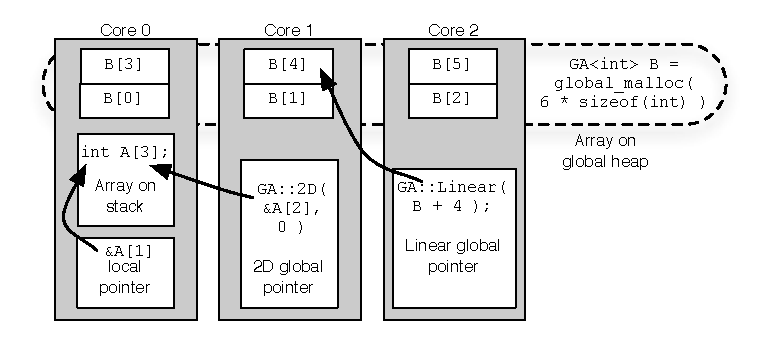
\includegraphics[width=0.95\columnwidth]{figs/memory-structure}
\begin{minipage}{0.95\columnwidth}
  \caption{\label{fig:memory-structure} Global memory referencing in \Grappa}
\end{minipage}
\vspace{-3ex}
\end{center}
\end{figure}

\paragraph{Global memory access} There are two general methods \Grappa
applications use to {\em access} global memory. One method is to use {\em
delegate} operations, which are short memory accesses performed at the memory
location's home node. This method is used when there is no locality in the
access. The other method is to do {\em explicit caching} of memory regions,
used when the programmer expects that the associated computation has data
locality. Below we explain each in detail.


\vspace{1ex} \textit{Delegate operations.} When the data access pattern has
low-locality, it is more efficient to modify the data on its home core rather
than bringing a copy to the requesting core and returning it after
modification. Delegate operations~\cite{Nelson:hotpar11, delegated:oopsla11}
provide this capability. Applications can dispatch computation to be performed
on individual machine-word sized chunks of global memory to the memory system
itself. Delegates are general, so we use them to perform simple
\emph{read\/}/\emph{write\/} operations to global memory, as well as more complex \emph{read-modify-write\/} operations (e.g., \emph{fetch-and-add\/}). 

Delegate operations are \emph{always\/} executed at the home core of their
address. The remote operation may not perform any operations that could cause
a context switch; this ensures any modifications are atomic. We limit delegate
operations to operate on objects in the 2D address space or objects that fit
in a single block of the linear address space so they can be satisfied with a
single network request. Given these restrictions, we can ensure that delegate
operations for the same address from multiple requesters are always serialized
through a single core in the system, providing atomic semantics without using
actual atomic operations (and thus avoiding their typical high cost).

Delegate operations can be either {\em synchronous} or {\em asynchronous}.
With synchronous operations, the task issuing the delegate call blocks until
the delegate operation completes, which is necessary, for example, to ensure
that synchronization has finished before continuing. Synchronization in \Grappa
is implemented using synchronous delegate operations. Often remote data
accesses do not need to be performed synchronously. In order to avoid
unnecessary waiting, we support asynchronous delegate operations. For reads,
we support a ``futures''-like mechanism. Tasks may issue delegate reads in
parallel and block on the ``promises'' returned by asynchronous delegate
invocations. Delegate write operations may also be performed asynchronously,
and since they do not return data, they need a mechanism to detect completion.
\Grappa provides a \texttt{GlobalCompletionEvent} object, which keeps track of
outstanding asynchronous operations of the local core. The code and can probe
the state of this object to determine when all outstanding requests are
complete. This is necessary to, say, make sure all outstanding operations are
complete before executing a synchronization operation.

\vspace{1ex}
\textit{Explicit caching.} \Grappa provides an API to fetch a global pointer of
any length and return a local pointer to a cached copy of the global memory.
\Grappa cache operations have the usual read-only and read-write variants,
along with a write-only variant used to initialize data structures. Languages
for distributed shared memory systems have done optimizations to achieve a
similar goal. For example, the UPC compiler coalesces struct and array
accesses into remote get/put \cite{Chen:2005}, and Fortran D compiler's
message vectorization hoists small messages out of a loop
\cite{FortranD:1992}. Caching in \Grappa additionally provides a mechanism for
exploiting temporal locality when available by operating on the data locally.

Under the hood, \Grappa performs the mechanics of gathering chunks of data from
multiple system nodes and presenting a conventional appearing linear block of
memory as a local pointer into a cache. The strategy employed is to issue all
the constituent requests of the desired block (as Active Messages) and then
yield until all responses have occurred. Currently, \Grappa caches are
\emph{not\/} kept coherent automatically. If that is desired, the programmer is
responsible for ensuring sufficient synchronization (via delegate operations)
occurs before acquiring or releasing cache objects.

Figure~\ref{fig:delegate-cache} depicts an example how explicit caching and
delegate operations work and how they interact.

\begin{figure*}[htb] \begin{center}
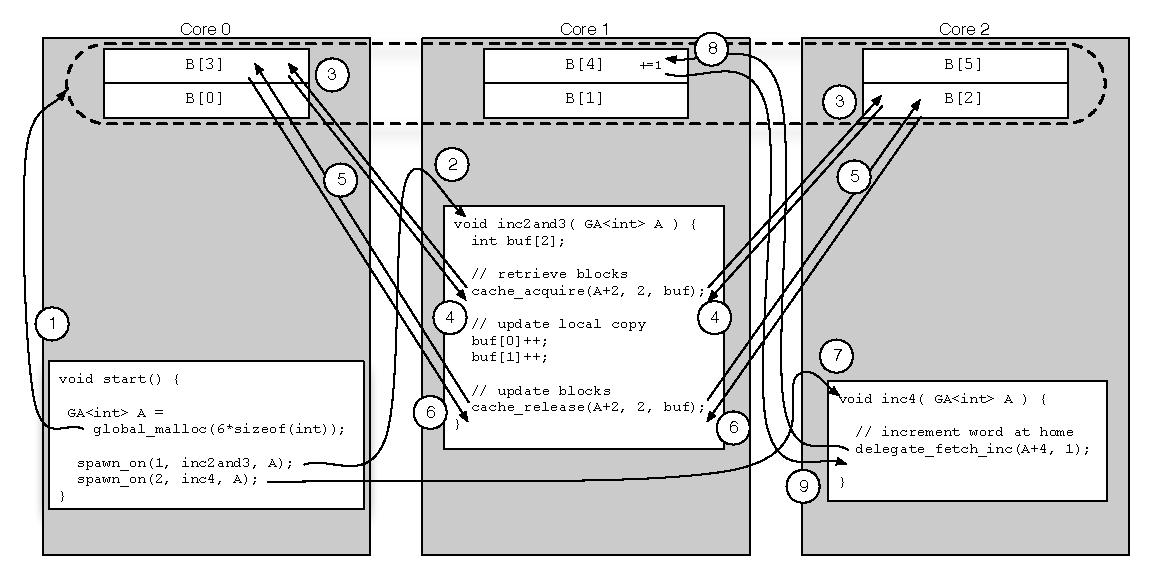
\includegraphics[width=1.5\columnwidth]{figs/delegate-cache}
\begin{minipage}{1.9\columnwidth} \caption{\label{fig:delegate-cache}
\textbf{Delegation and cache example:} A core allocates an array in the global
heap (1). It then spawns two tasks on remote cores to increment elements of
the array. The first task increments two elements of the array using cache
operations. The first task is then invoked (2). A cache request is issued for two
adjacent integers starting at the second element of the array. Since these
element are stored in the memories of two different cores, this requires two messages to be sent (3). The task is suspended until both responses arrive
(4). The data carried in these responses is stored in the local buffer. The
elements are then incremented in the buffer. The modified data is then sent back
to the home node (5). Acknowledgements are returned (6) so the task
knows when the writes are complete. The second task increments an element of
the array with a delegate operation. The task is invoked (7). A delegate
request is sent to the home core of the array element with the increment
value. The task suspends until the response is received. The increment
is executed on the remote core (8). A response is returned (9) with the
previous value of the array element. } \end{minipage} \vspace{-3ex}
\end{center} \end{figure*}

\paragraph{Memory consistency model discussion} As mentioned earlier, all
synchronization operations are done via delegate operations. Since they all
execute in their home node, they are guaranteed to be serialized, with their
updates visible to all cores across the system in the same order. Also, tasks
are restricted to a single outstanding synchronous delegate operation at a
time, which is how synchronization is done. Therefore, synchronization operations are not subject to potential reordering. 
% \TODO{I think we can support multiple delegates in parallel from a task as
% long as we block on them before counting on them being complete. see my
% description above about the \emph{future/promise} delegates we have now. Not
% sure if there's a strong example of when this is useful for synchronization
% (though it's definitely useful for reads/writes), acquiring multiple locks
% doesn't work because we have to acquire locks in order to prevent deadlock.}
Consequently, all synchronization operations execute in program order and are
made visible in the same order to all cores in the system. These properties
are sufficient to guarantee a memory model that offers sequential consistency
for data-race-free programs~\cite{AdveHill1990} (all accesses to shared data
are separated by synchronization). This is the memory model that underpins
C/C++~\cite{N2480,N2800}.

Note, however, that if the application code uses explicit caching or
asynchronous delegates to access shared data, all updates must be sent back to
the home node before the synchronization operation that protects the data is
performed. This is done using release operations on cached regions and using
the \texttt{GlobalCompletionEvent} object to determine that asynchronous
delegates have been fully executed.




